\documentclass[tikz,border=10pt]{standalone}
% Scale: s = 0.014706 cm per px (from STYLE METRICS), origin at O
\begin{document}
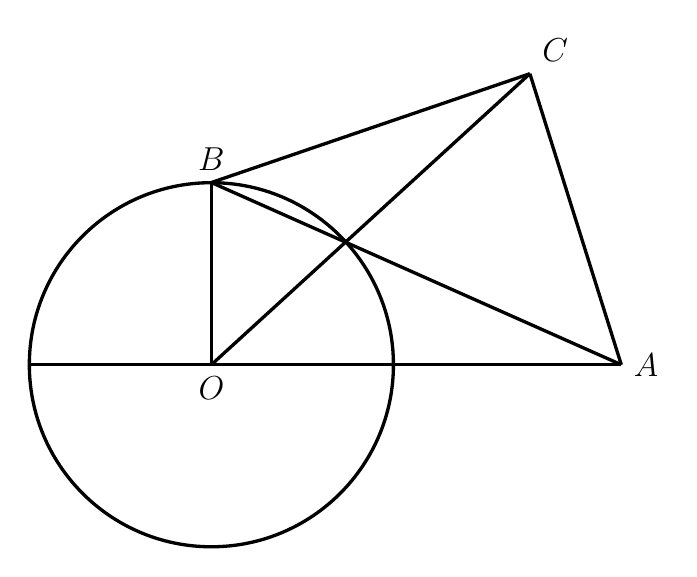
\begin{tikzpicture}[line join=round, line width=1.2pt]
  % Named coordinates (units = cm)
  \coordinate (O) at (0,0);
  \coordinate (A) at (5.206,0);       % A on x-axis
  \coordinate (B) at (0,2.314);       % B on circle top
  \coordinate (C) at (4.045,3.696);   % C
  \coordinate (L) at (-2.312,0);      % circle left point
  \coordinate (P) at (1.702,1.559);   % interior point on BA and CO

  % Circle centred at O, radius 2.312
  \draw (O) circle (2.312);

  % Horizontal line from left circle point through O to A
  \draw (L) -- (A);

  % Remaining segments
  \draw (O) -- (B);   % vertical OB
  \draw (C) -- (O);   % CO
  \draw (B) -- (A);   % BA
  \draw (C) -- (B);   % CB
  \draw (C) -- (A);   % CA

  % Labels
  \fontsize{12.5}{15}\selectfont
  \node[above right] at (C) {$C$};
  % B: directly above vertex B, centred on its x-coordinate
  \node[above] at (B) {$B$};
  \node[right]       at (A) {$A$};
  % O: directly below the origin, centred under it
  \node[below] at (O) {$O$};
\end{tikzpicture}
\end{document}